\chapter{Arquitetura do sistema}

\begin{figure}[htbp]
\centering
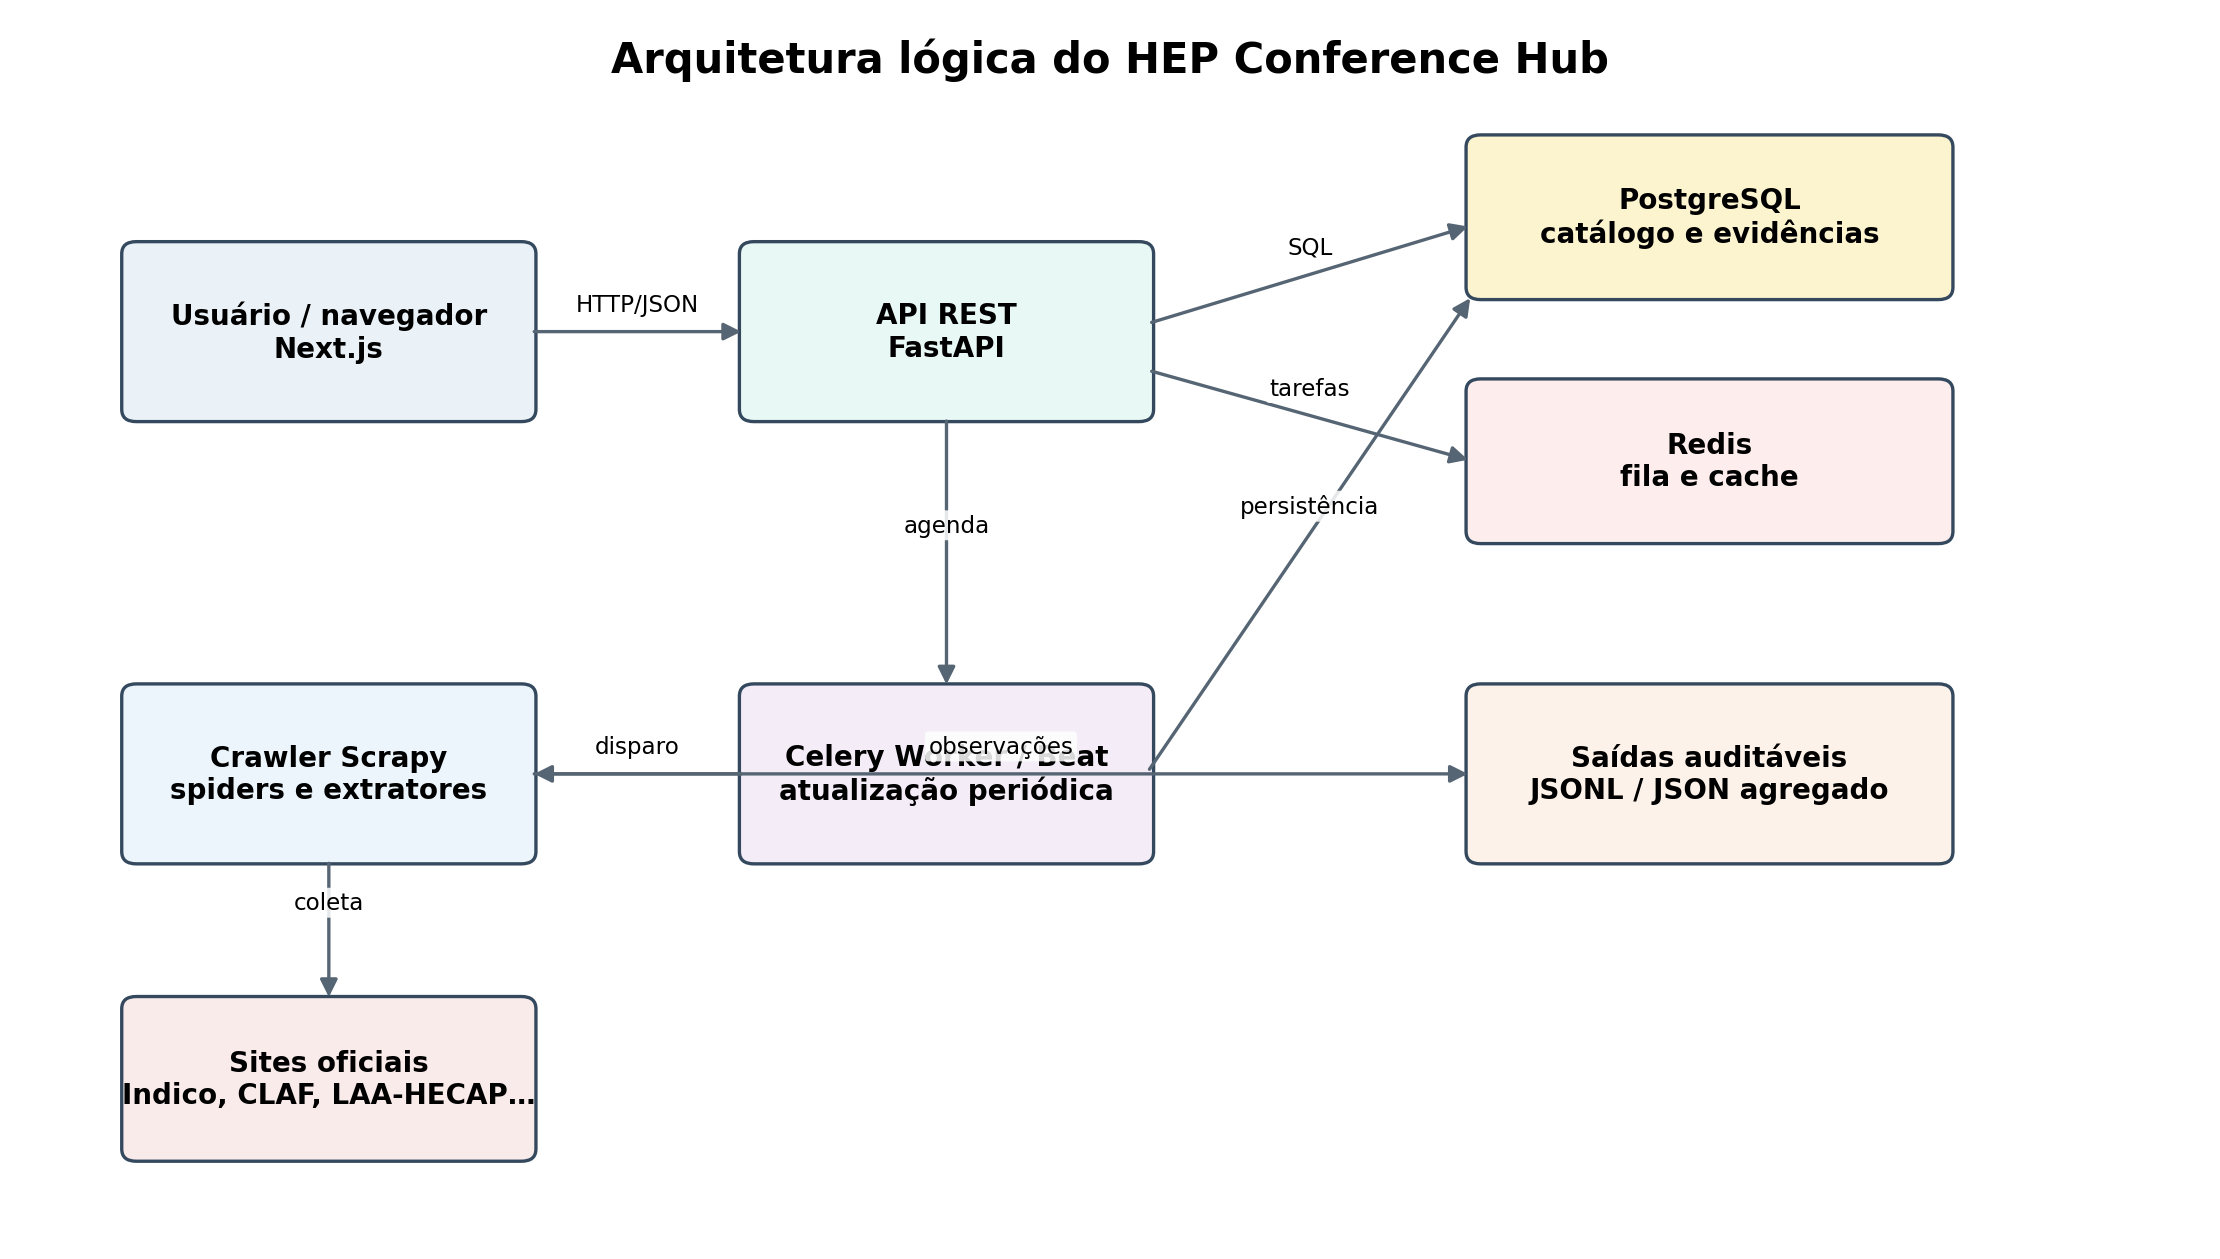
\includegraphics[width=\textwidth]{figuras/arquitetura_logica.png}
\caption{Arquitetura lógica do portal.}
\end{figure}

A solução adota arquitetura distribuída em serviços, coordenada por Docker Compose. O navegador acessa o frontend Next.js, que consome a API FastAPI. A API persiste dados em PostgreSQL e despacha tarefas por Redis/Celery. O crawler Scrapy visita fontes oficiais, produz observações auditáveis e alimenta o processo de normalização e persistência.

\section{Serviços principais}

\begin{center}
\small
\renewcommand{\arraystretch}{1.15}
\begin{longtable}{>{\RaggedRight\arraybackslash}p{0.16\textwidth}>{\RaggedRight\arraybackslash}p{0.25\textwidth}>{\RaggedRight\arraybackslash}p{0.51\textwidth}}
\toprule
\textbf{\textbf{Serviço}} & \textbf{\textbf{Responsabilidade}} & \textbf{\textbf{Porta/Canal}} \\
\midrule
\endfirsthead
\toprule
\textbf{\textbf{Serviço}} & \textbf{\textbf{Responsabilidade}} & \textbf{\textbf{Porta/Canal}} \\
\midrule
\endhead
\midrule
\multicolumn{3}{r}{\footnotesize Continua na próxima página} \\
\endfoot
\bottomrule
\endlastfoot
web & Interface web, filtros, cartões e painéis de auditoria. & 3000/TCP \\
api & Endpoints REST, regras de negócio, schemas e persistência. & 8000/TCP \\
postgres & Banco relacional e armazenamento persistente. & 5432/TCP \\
redis & Broker para Celery e possível cache. & 6379/TCP \\
worker & Execução assíncrona de atualização e processamento. & Fila Redis \\
beat & Agendamento periódico das tarefas. & Fila Redis \\
crawler & Coleta externa sob demanda ou acionada por tarefa. & HTTP/HTTPS externo \\
\end{longtable}
\end{center}

\section{Fluxo de dados}

\begin{figure}[htbp]
\centering
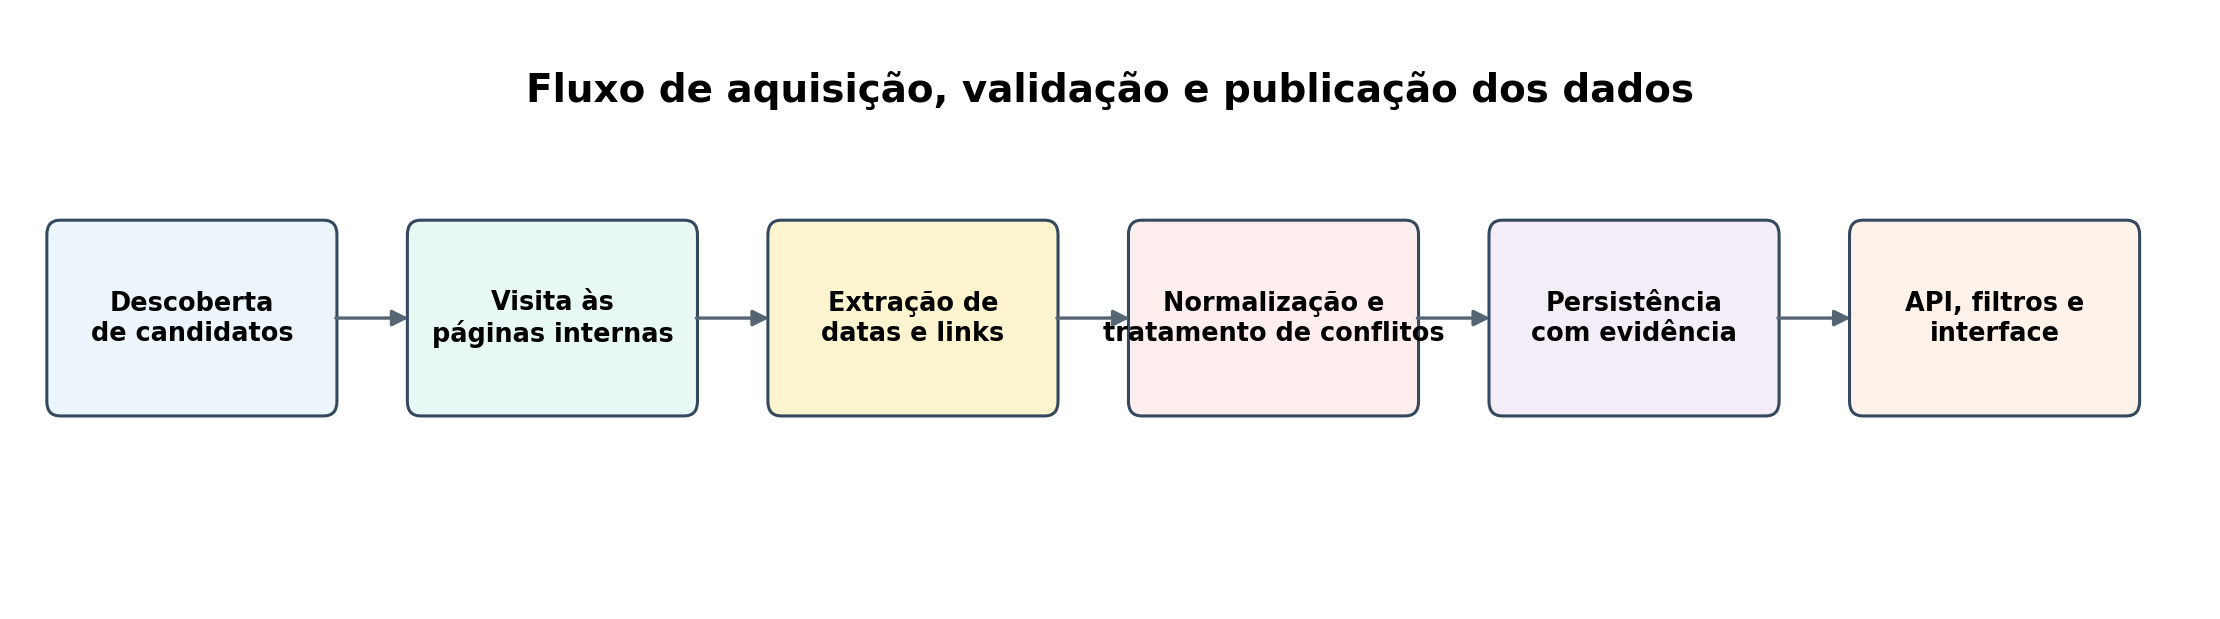
\includegraphics[width=\textwidth]{figuras/fluxo_aquisicao_publicacao.png}
\caption{Fluxo da descoberta à publicação.}
\end{figure}
